\documentclass[a4paper,12pt]{article}
\usepackage{color}
\usepackage{amsmath} % do fancy math
\usepackage{mathtools}
\usepackage{amsfonts}
\usepackage{bm}
\usepackage{amsthm} % math theorem proof etc
\usepackage{graphicx} % import images
\usepackage{tikz} % draw images with latex
\usepackage{pgf} % go with tikz
\usepackage{subfigure}
\usepackage{caption}
\usepackage{multirow}
\usepackage{algorithm}
\usepackage{algorithmic}
\usepackage{epstopdf}
\usepackage[round]{natbib}
\usepackage{setspace}
\usepackage[top=30mm, bottom=30mm, left=35mm,right=30mm]{geometry}
\usepackage[utf8]{inputenc}
\usepackage[acronym]{glossaries}
\newcommand{\ud}{\,\mathrm{d}}
%% Compilation need terminal
%pdflatex glossaries.tex
%makeglossaries glossaries
%pdflatex glossaries.tex

\makeglossaries

\newglossaryentry{fwmodel}
{
        name=forward model,
        description={physical model, usually a (partial) differential equation system, used to
                     solve certain geophysical process}
}
\newglossaryentry{fwmodelling}
{
        name=forward modelling,
        description={The approach that link the process contribution to the corresponding observation.}
}
\newglossaryentry{footprint}
{
        name=foot print,
        description={The spatial unit where the geophysical process makes a contribution to the observed data.}
}

\newglossaryentry{hyperpars}
{
        name=hyper parameters,
        description={parameters in defining the covariance structure of the latent process; in particular for a Gaussian process with Mat\'{e}rn
                        covariance function, the hyper parameters are the \gls{lengthscale} $\rho$ and \gls{normvar} $\sigma^2$}
}
 
\newglossaryentry{lengthscale}
{
        name=lengthscale,
        description={define and usually denoted by $\rho$}
}

\newglossaryentry{mesh}
{
        name=mesh,
        description={A triangulation of a given area.}
}
 
\newglossaryentry{normvar}
{
        name=norminal variance,
        description={usually denoted by $\sigma^2$}
}

\newglossaryentry{predmean}
{
        name=predicted mean,
        description={the mean with respect to the predictive distribution}
}
\newglossaryentry{preduncert}
{
        name=predicted uncertainty,
        description={the standard deviation with respect to the predictive distribution}
}
\newglossaryentry{predist}
{
        name=predictive distribution,
        description={the posterior marginal distribution of a given location $X_i$ that integrate out the unknown parameters and $\bm{X_{-i}}$}
}



\newglossaryentry{prior}
{
        name=prior distribution,
        description={the probability distribution for the (hyper) parameters or latent processes}
}

\newglossaryentry{priorinfo}
{
        name=prior information,
        description={information for setting up the model, including the values for the parameters,
                     constraints,  etc.}
}

\newacronym{bhm}{BHM}{Bayesian hierarchical model} 
\newacronym{cosp}{COSP}{change of support problem} 
\newacronym{gia}{GIA}{glacial isostatic adjustment}
\newacronym{gp}{GP}{Gaussian process}
\newacronym{gmrf}{GMRF}{Gaussian Markov random field}
\newacronym{iid}{iid}{independent identically distributed}
\newacronym{spde}{SPDE}{stochastic partial differential equation}
\newacronym{inla}{INLA}{integrated nested Laplace approximation}
\newacronym{mcmc}{MCMC}{Markov chain Monte Carlo}
\newacronym{pdf}{pdf}{probability density function}

\begin{document}
 \title{GlobalMass project glossary}
\author{The GlobalMass Team\footnote{Z. Sha contributes to most part of the Bayesian Hierarchical model.}}
\maketitle

\onehalfspacing
\numberwithin{equation}{section}


\section{The Bayesian hierarchical model}
In this section, we introduce the Bayesian hierarchical model for predicting the global \acrshort{gia} process. 

We assume that the true \acrshort{gia} process is a real-valued spatial process continues on the sphere and denote it by $\bm{Y}: \mathbb{S}^2 \mapsto \mathbb{R}$. We use one of the \acrshort{gia} solution, say from one of the \emph{ice6g} models, as the prior mean of the true process and denote it by $\bm{\mu}: \mathbb{S}^2 \mapsto \mathbb{R}$. Then the residuals between the true process and \gls{fwmodel} solutions can be modelled as a stationary Gaussian process on the sphere 
\begin{align}\label{eq:GIAresid}
 \bm{X}: = \bm{Y} - \bm{\mu} \sim \mathcal{GP}(\bm{0}, \kappa(\bm{\theta}))
\end{align}
where $\kappa(\bm{\theta})$ defines the covariance function with \gls{hyperpars} $\bm{\theta}$.

In order to assess the bias and uncertainties in the \emph{ice6g} solutions, we use the GPS observations to update the \acrshort{gia} process. The GPS  data are the yearly trends of vertical movements in millimetre at the observed locations. These observations can be regarded as a linear map of the \acrshort{gia} process with measurement errors.

\subsection{From geophysical processes to observations}
With the geophysical processes defined and data processed, we need to link the processes to various observations according to their contributions. These links are usually linear translators that average the process values at the different spatial scales of the data. This is often called \emph{\acrfull{cosp}} in the literature of spatial statistics. 

In our framework, we define the term spatial \emph{\gls{footprint}} $\Omega_i$ of an observation $O_i$ as the spatial unit where the geophysical process has a contribution to the observed value. Define $\bm{\mathcal{A}_i}$ to be a linear operator that maps from the process value over $\Omega_i$ to the observation value $O_i$ over its own spatial unit $\delta_i$. Then $\bm{\mathcal{A}_i}$ can usually be a map from point to point, area to point or area to area. Figure \ref{fig:footprint} shows the footprint of the GPS and GIA data.
\begin{figure}[hbtp]
\centering
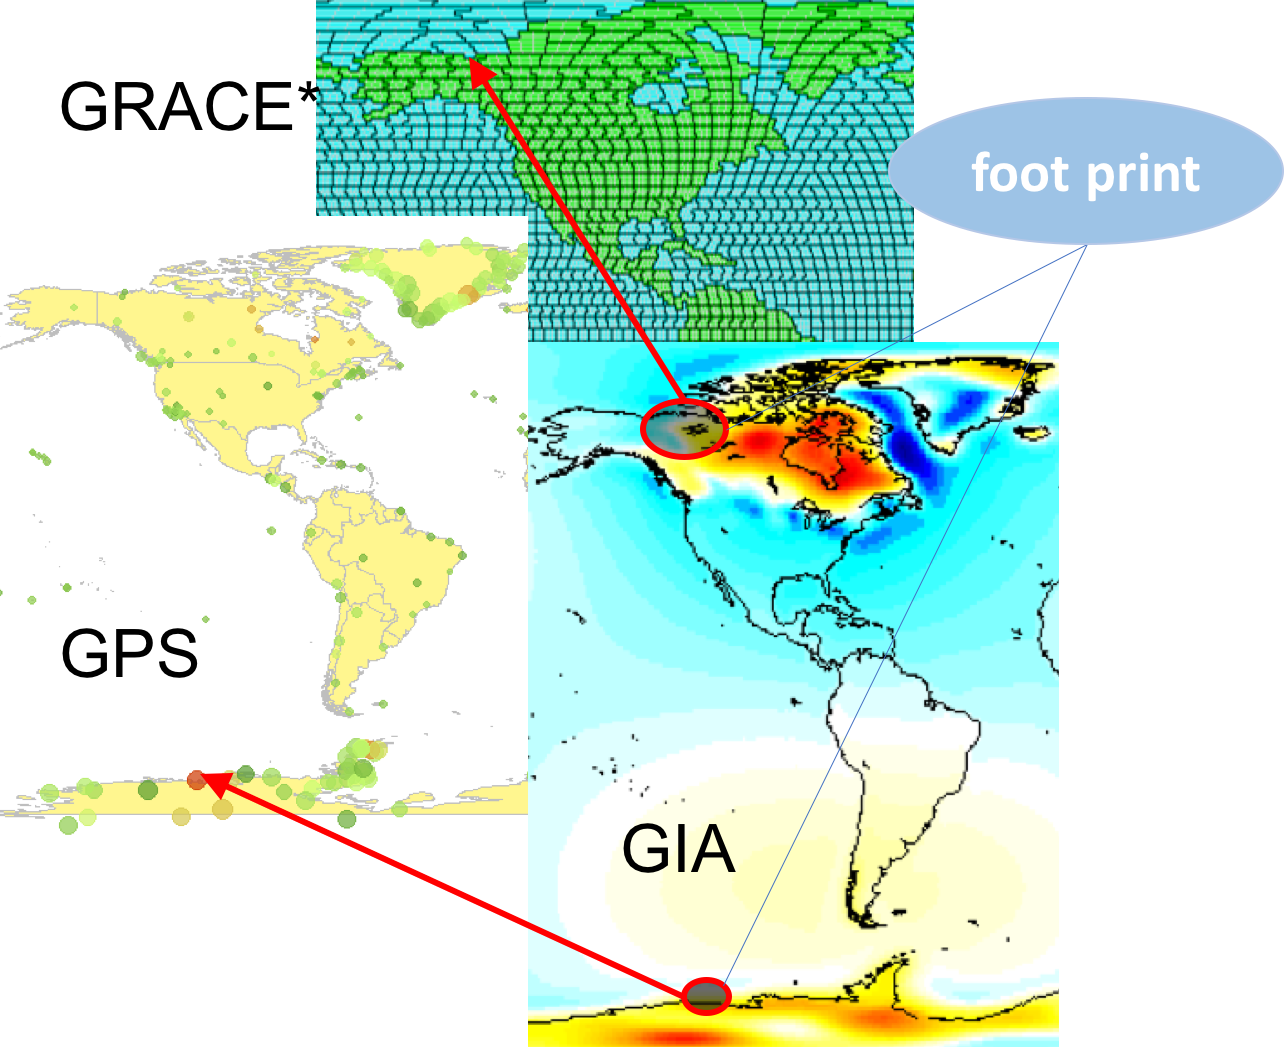
\includegraphics[width= 0.7\textwidth]{footprint}
\caption{Examples of foot prints of GPS and GRACE data on the GIA process.}\label{fig:footprint}
\end{figure}


For example, the GPS signal can be affected by GIA process over a large area with decaying weights along distance to the GPS location. In this first test of framework, we simple assume the foot print of a GPS data point to be a single point of the GIA process at the same location. Thus, $\mathcal{A}_i$ is a point to point map and we have the following observation equation
\begin{align}\label{eq:GPSi}
Z_i = \bm{\mathcal{A}}_i\bm{Y} + \varepsilon_i, \; i = 1,\dots N.
\end{align} 
where $Z_i$ measures the uplift rate of the bedrock at the $i^{th}$ GPS station and the measurement errors $\varepsilon_i$s are assumed to be independent Gaussian errors $\mathcal{N}(0, e_i^2)$. In practice, $Z_i$ is estimated from the raw GPS time series signals and $e_i$ is fixed to be the standard error $Z_i$. 

Then by stacking $\bm{\mathcal{A}_i}$ together as 
\begin{align*}
\bm{\mathcal{A}} = \left[\begin{array}{c}
 \bm{\mathcal{A}}_1\\ \vdots \\ \bm{\mathcal{A}}_N \end{array} \right],
\end{align*}
we can write equation \eqref{eq:GPSi} into vector form
\begin{align}\label{eq:GPS}
\bm{Z} = \bm{\mathcal{A}}\bm{Y} + \bm{\varepsilon} 
\end{align}

Now combining equations \eqref{eq:GIAresid} and \eqref{eq:GPS}, the system simplifies to
\begin{align}
\bm{\tilde{Z}} = \bm{Z} - \bm{\mathcal{A}}\bm{\mu}= \bm{\mathcal{A}}\bm{X} + \bm{\varepsilon}
\end{align}
Hence, our final model is
\begin{align}
\left\{ \begin{array}{l}
\bm{\tilde{Z}} = \bm{\mathcal{A}}\bm{X} + \bm{\varepsilon}, \; 
\bm{\varepsilon} \sim \mathcal{N} (\bm{0}, \mbox{diag}(e_1^2, e_2^2, \dots, e_N^2)) \\
\bm{X} \sim \mathcal{GP}(\bm{0}, \kappa(\bm{\theta})) \\
\bm{\theta} \sim \bm{p}(\bm{\theta})
\end{array} \right.
\end{align}
where $\bm{\pi}(\bm{\theta})$ is the \gls{prior} for the \gls{hyperpars}.

We call the above approach of linking the process to the observation \emph{\gls{fwmodelling}}. To be differentiated from \gls{fwmodel}, the \gls{fwmodelling} approach describes the functional relationship between the process and the data rather than the underlying physical mechanism of the latent process.

\subsection{GMRF Approximation}
Suppose we would like to predict the \acrshort{gia} process on a set of grid points $\bm{S} = \{s_i: i = 1,\dots, m\}$ with a given resolution. The Gaussian process model can be computationally expensive for large scale inference since the Bayesian update scales as $\mathcal{O}(m^3)$ mainly due to the inverse of a dense covariance matrix. 

At the same time, \acrlong{gmrf} is often used for modelling discrete spatial unit. The covariance structure is defined through its inverse, the precision matrix, which is usually sparse and thus has nice computational properties.

The Gaussian process with Mat\'{e}rn covariance function can be treated as solutions to a class of \acrlong{spde}s \citep{Lindgren2011} which can then be approximated by \acrshort{gmrf} using finite element methods. 

Denote by $\bm{\tilde{X}}$ the \acrshort{gmrf} approximation of $\bm{X}$ on a given triangulation of the sphere with piecewise linear local basis functions $\{ \bm{\phi}_i \}_{i \in \mathbb{N}}$, then given any location $s \in \mathbb{S}^2$
\begin{align}
\bm{X}(s) \approx \bm{\phi}_i(s)^T\bm{\tilde{X}}
\end{align}
and for a given set $\bm{S}$ of locations, we have  
\begin{align}
\bm{X}(\bm{S}) \approx \bm{C}(\bm{S})\bm{\tilde{X}}
\end{align}
where the matrix $\bm{C}$ contains basis functions for all locations.

Now with the GMRF approximation, our model becomes
\begin{align}
\left\{ \begin{array}{l}
\bm{\tilde{Z}} = \bm{\mathcal{A}}\bm{C}\bm{\tilde{X}} + \bm{\varepsilon}, \; 
\bm{\varepsilon} \sim \mathcal{N} (\bm{0}, \mbox{diag}(e_1^2, e_2^2, \dots, e_N^2)) \\
\bm{\tilde{X}} \sim \mathcal{N}(\bm{0}, \bm{Q}^{-1}(\bm{\theta})) \\
\bm{\theta} \sim \bm{p}(\bm{\theta})
\end{array} \right.
\end{align}
where $\bm{Q}$ is the precision matrix of the \acrshort{gmrf} approximation.

The \acrshort{gmrf} approximation requires generating a \gls{mesh} which is often a triangulation of a given area of interest. Then $\bm{\tilde{X}}$ are located at the vertices of the mesh. For a mesh that is approximately regular, we define the resolution of the mesh to be the average area of the triangles converted to degree by degree; and for irregular mesh, the resolution is calculated by using the smallest triangle.

\subsection{Bayesian Inference and prediction}
The Bayesian inference requires finding the posterior distributions of the hyper parameters and the latent process. The \acrfull{mcmc} can be used in general to sample from the posteriors and the \acrfull{inla} is a fast approximation method. In the following, we use $\bm{\pi}$ for a general \acrshort{pdf} and define a few terms used in our Bayesian inference.

The Bayesian inference draw conclusions from the posterior distribution 
\begin{align}
\bm{\pi}(\bm{X}, \bm{\theta} | \bm{\tilde{Z}}) = \frac{\bm{\pi}(\bm{X},\bm{\theta}, \bm{\tilde{Z}})}{\bm{\pi}(\bm{\tilde{Z}})}
=\frac{\bm{\pi}(\bm{\tilde{Z}}| \bm{X}, \bm{\theta}) \bm{\pi}(\bm{X}|\bm{\theta})\bm{\pi}(\bm{\theta})}
{\int_{\bm{\mathcal{X}}, \bm{\Theta}}\bm{\pi}(\bm{\tilde{Z}}| \bm{X}, \bm{\theta}) \bm{\pi}(\bm{X}|\bm{\theta})\bm{\pi}(\bm{\theta})\ud\bm{X} \ud\bm{\theta}}
\end{align}
This is the joint distribution of the latent process and the hyper parameters but in practice we are more interested in the posterior marginals for inference on parameters and prediction of the latent filed separately. For simplicity, we use posterior distribution for 
\begin{align}
\bm{\pi}(\bm{\theta}| \bm{\tilde{Z}}) = 
\int_{\bm{\mathcal{X}}} \bm{\pi}(\bm{X}, \bm{\theta} | \bm{\tilde{Z}}) \ud \bm{X}
\end{align}
the posterior marginal distribution for the hyper parameters. Inference on the parameters is not of crucial importance here but provides as sanity checks for the process property such as the length of spatial correlation. The aim of the study is to predict the latent process and the corresponding uncertainty on a fine resolution map; hence define the joint predictive distribution of the latent process to be 
\begin{align}
\bm{\pi}(\bm{X}| \bm{\tilde{Z}}) = 
\int_{\bm{\Theta}} \bm{\pi}(\bm{X}, \bm{\theta} | \bm{\tilde{Z}}) \ud \bm{\theta}
\end{align}
the posterior marginal distribution of the latent process that integrate out the uncertainty of the hyper parameters. In practice, we are more interested in predicting the marginal means and variances  at a given set of locations; hence we define the point-wise \gls{predist} to be 
\begin{align}
\bm{\pi}(X_i | \bm{\tilde{Z}}) = \int_{\bm{\mathcal{X}_{-i}}} \bm{\pi}(\bm{X} | \bm{\tilde{Z}}) \ud \bm{X_{-i}}
\end{align}
where $X_i$ is the latent process at location $i$ and $\bm{X_{-i}}$ are $\bm{X}$ elsewhere. The \gls{predmean} $X_i^*$ and \gls{preduncert} $\mbox{u}(X_i)$ are the expectation and standard deviation with respect to $\bm{\pi}(X_i | \bm{\tilde{Z}})$
\begin{align}
&X_i^* = \mathbb{E}(X_i| \bm{\tilde{Z}}) = 
\int_{\mathbb{R}} X_i \bm{\pi}(X_i | \bm{\tilde{Z}}) \ud X_i \\
&\mbox{u}(X_i) = \sqrt{\mbox{Var}(X_i| \tilde{Z})} = \sqrt{\int_{\mathbb{R}} (X_i - X_i^*)^2\bm{\pi}(X_i | \bm{\tilde{Z}}) \ud X_i}
\end{align}

The \acrshort{inla} method directly approximate the $\bm{\pi}(X_i | \bm{\tilde{Z}})$ and provide the predicted mean and uncertainty as summary statistics. For the \acrshort{mcmc} approach, the \gls{predist} can be approximate by the posterior sample distribution of $X_i$ and the \gls{predmean} and \gls{preduncert} by the sample mean and standard error.

\acrshort{inla} is much faster and more efficient than MCMC in providing the \gls{predist} but it provides limited information on the joint posterior distributions. The MCMC samples can be used in various ways for exploring the posteriors.



\clearpage
 
\printglossary[type=\acronymtype]
 
\printglossary
 
\bibliographystyle{abbrvnat}
\bibliography{references}

\end{document}